\documentclass[a4paper, 11pt]{article}
\usepackage{amsmath}
\usepackage{graphicx}
\usepackage{geometry}
\usepackage{listings}
\geometry{scale=0.8}
\linespread{1.5}
\usepackage{hyperref}

\title{	
\normalfont \normalsize
\textsc{School of Data and Computer Science, Sun Yat-sen University} \\ [25pt] %textsc small capital letters
\rule{\textwidth}{0.5pt} \\[0.4cm] % Thin top horizontal rule
\huge  P02  CSP and KRR\\ % The assignment title
\rule{\textwidth}{2pt} \\[0.5cm] % Thick bottom horizontal rule
\author{Yikun Liang}
\date{\normalsize\today}
}

\begin{document}
\maketitle
\tableofcontents
\newpage




\section{Futoshiki (GAC, C++/Python)}
\subsection{Description}
Futoshiki is a board-based puzzle game, also known under the name Unequal. It is playable on a square board having a given fixed size ($4\times4$ for example), please see Figure \ref{fig:futoshiki}.

The purpose of the game is to discover the digits hidden inside the board's cells; each cell is filled with a digit between 1 and the board's size. On each row and column each digit appears exactly once; therefore, when revealed, the digits of the board form a so-called Latin square.

At the beginning of the game some digits might be revealed. The board might also contain some inequalities between the board cells; these inequalities must be respected and can be used as clues in order to discover the remaining hidden digits.

Each puzzle is guaranteed to have a solution and only one.

You can play this game online: \url{http://www.futoshiki.org/}.
\begin{figure}[h]
  \centering
  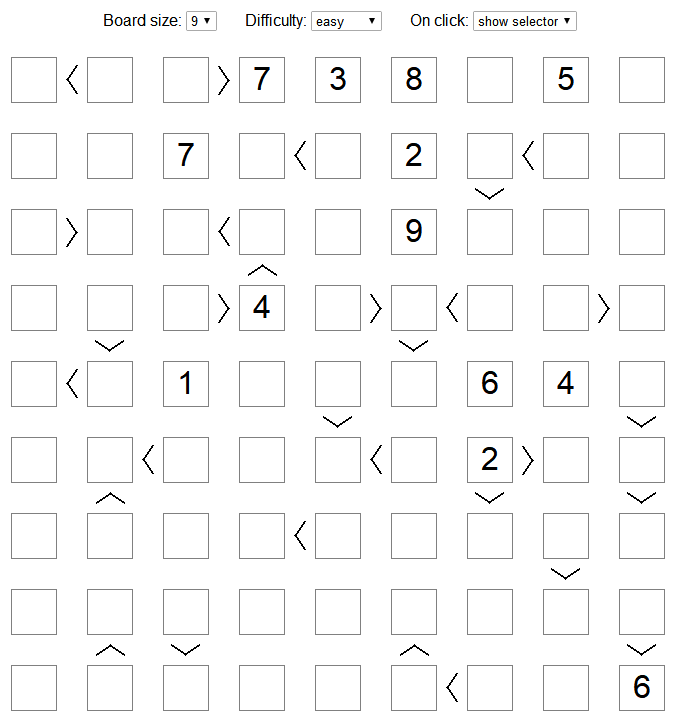
\includegraphics[width=6cm]{Pic/futoshiki1}
  \qquad
  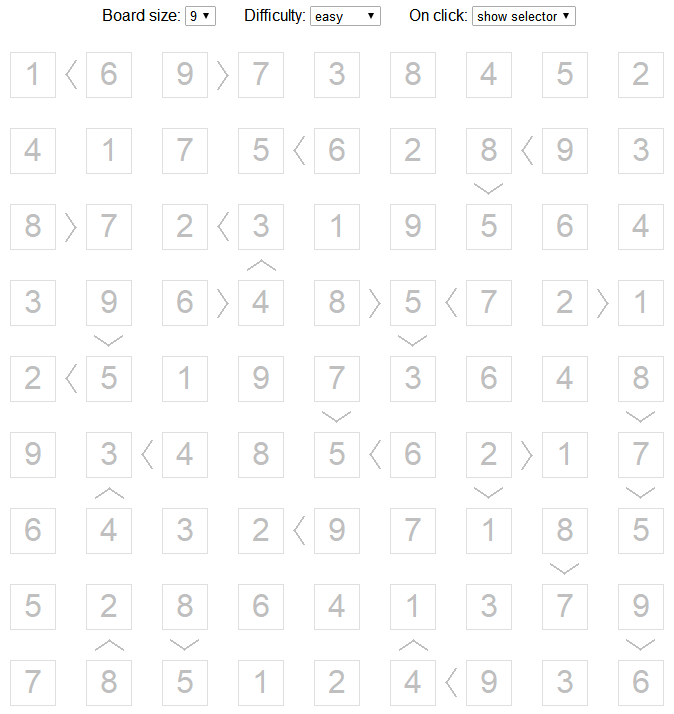
\includegraphics[width=6cm]{Pic/futoshiki2}
  \caption{Futoshiki Puzzles}
  \label{fig:futoshiki}
\end{figure}

\subsection{Tasks}

\begin{enumerate}
\item You should use \textbf{GAC} algorithm to implement a Futoshiki solver by \textbf{C++} or \textbf{Python}.
\item If necessary, you could add some heuristic strategies to speed up your algorithm. 
\item You should run the following 5 test cases to verify your solver's \textbf{correctness} and \textbf{efficiency} in Figure \ref{fig:case11}, \ref{fig:case22}, \ref{fig:case33}, \ref{fig:case44}, and \ref{fig:case55}, and I will grade your codes in \textbf{GAC implementation}, \textbf{correctness of 5 cases} and \textbf{algorithm efficiency}.
\item Don't forget you have implemented this game by FC algorithm in E04.
    \begin{figure}[htbp]
    \centering
    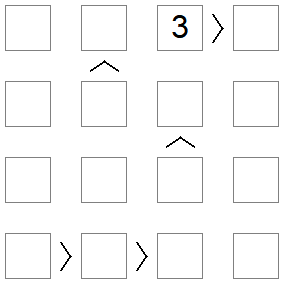
\includegraphics[width=6cm]{Pic/f1}
    \qquad
    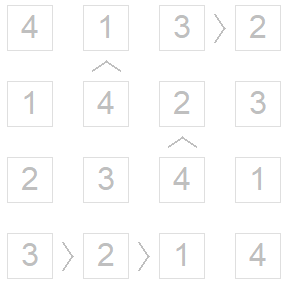
\includegraphics[width=6cm]{Pic/f1s}
    \caption{Futoshiki Test Case 1}
    \label{fig:case11}
  \end{figure}
        \begin{figure}[htbp]
    \centering
    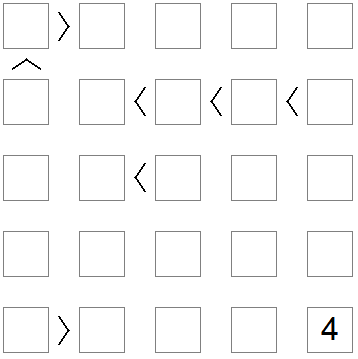
\includegraphics[width=6cm]{Pic/f2}
    \qquad
    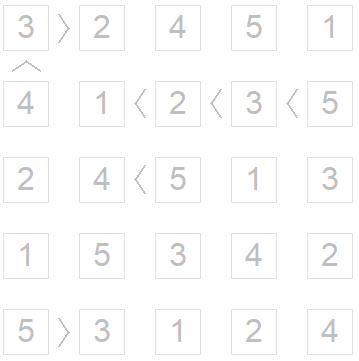
\includegraphics[width=6cm]{Pic/f2s}
    \caption{Futoshiki Test Case 2}
    \label{fig:case22}
  \end{figure}
        \begin{figure}[htbp]
    \centering
    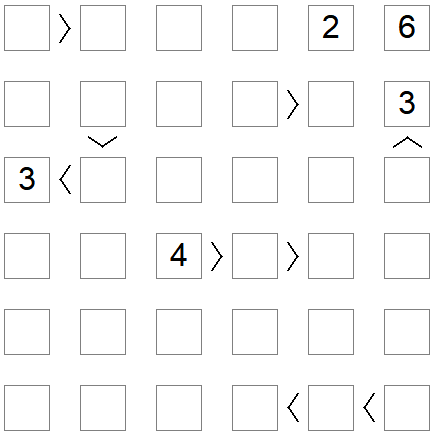
\includegraphics[width=6cm]{Pic/f3}
    \qquad
    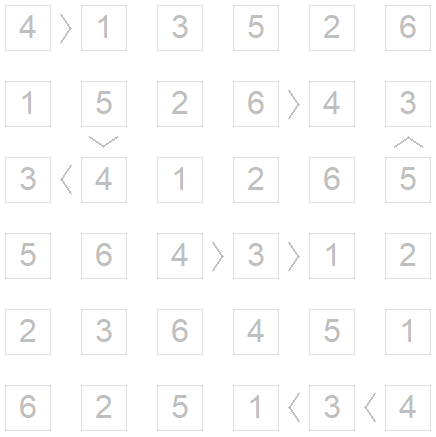
\includegraphics[width=6cm]{Pic/f3s}
    \caption{Futoshiki Test Case 3}
    \label{fig:case33}
  \end{figure}
        \begin{figure}[htbp]
    \centering
    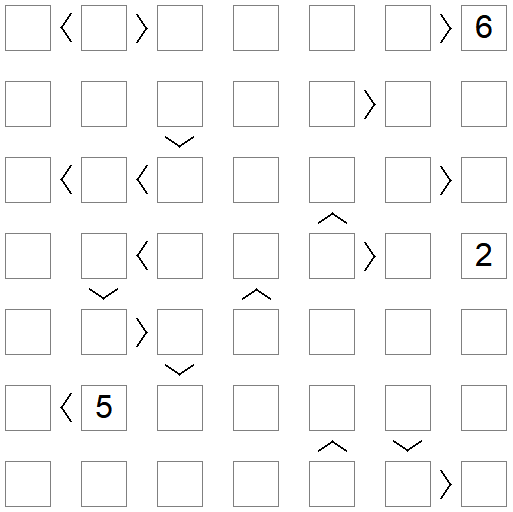
\includegraphics[width=7.5cm]{Pic/f4}
    \qquad
    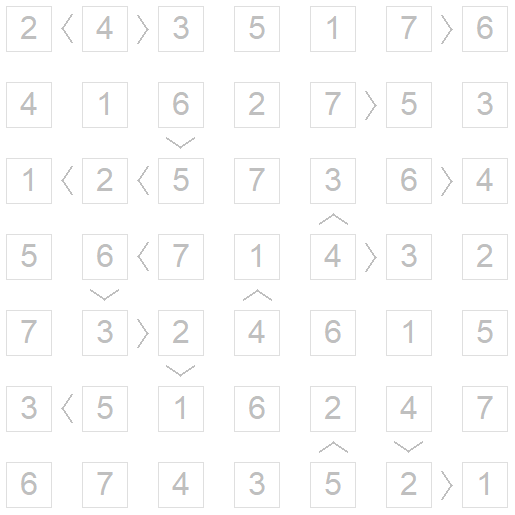
\includegraphics[width=7.5cm]{Pic/f4s}
    \caption{Futoshiki Test Case 4}
    \label{fig:case44}
  \end{figure}
        \begin{figure}[htbp]
    \centering
    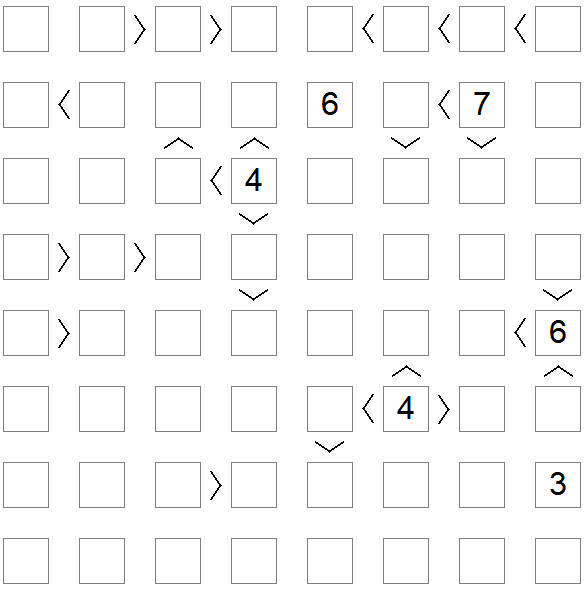
\includegraphics[width=7.5cm]{Pic/f5}
    \qquad
    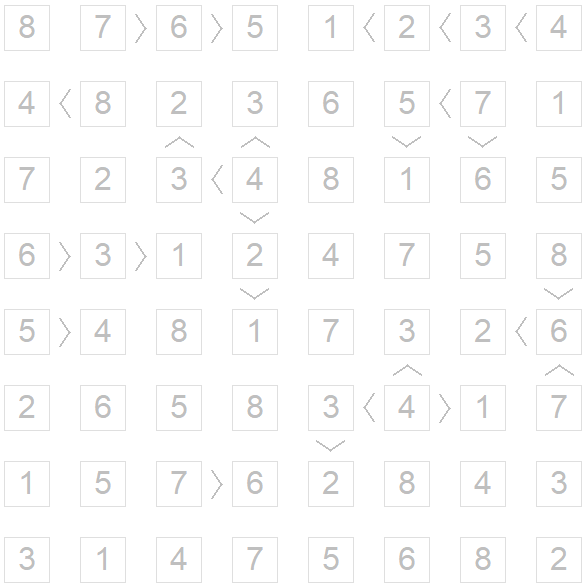
\includegraphics[width=7.5cm]{Pic/f5s}
    \caption{Futoshiki Test Case 5}
    \label{fig:case55}
  \end{figure}

\end{enumerate}

\section{Blocks World (Planner, Prolog)}
\subsection{Description}
Planning in the blocks world is a traditional planning exercise, and you can recall what we have introduced in class in Figure \ref{fig:blocks}:
\begin{figure}[ht]
\centering
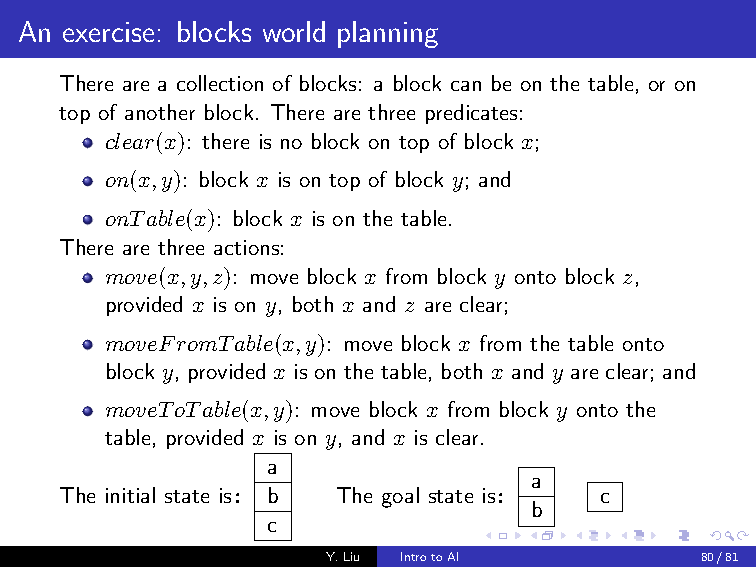
\includegraphics[width=13cm]{Pic/blocks}
\caption{Blocks World}
\label{fig:blocks}
\end{figure}

Here are several hints for you to develop a blocks world planner by using Prolog:
\begin{itemize}

  \item You can represent the states with \texttt{on(Block,Object)} and \texttt{clear(Object)}. You'd better take into account the location of the blocks, so \texttt{Objection} can be a block or a place.
  \item The only kind of action can be \texttt{move(Block,From,To)}.
  \item Each available action is defined in terms of its precondition and its effects. Preconditions can be defined by the procedure \texttt{can(Action,Cond)}. The effects of an action can be defined by two procedures:\texttt{adds(Action,AddRels)} and \texttt{deletes(Action,DelRels)}.
  \item The planner aims at finding a plan, that is, a sequence of actions, which achieves the goal. You can adopt the principle of planning by means-ends analysis illustrated in Figure \ref{fig:means_ends}:
  \item In order to delete unnecessary steps, you can consider avoiding those actions that destroy goals.

\end{itemize}
\begin{figure}[ht]
    \centering
    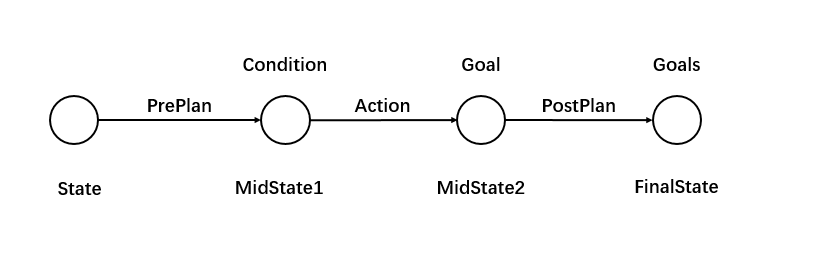
\includegraphics[width=17cm]{Pic/means_ends}
    \caption{The Principle of Means-Ends Planning}
    \label{fig:means_ends}
\end{figure}


\subsection{Tasks}
\begin{itemize}
    \item Please develop a planner to solve the blocks world problem by using Prolog. 
    \item There are 5 cases (Figure \ref{fig:blocks1}, Figure \ref{fig:blocks2}, Figure \ref{fig:blocks3}, Figure \ref{fig:blocks4} and Figure \ref{fig:blocks5}) for you to test the performance of your planner. I will grade your planner in \textbf{correctness of cases}, \textbf{the number of steps}, and \textbf{time cost}. 
    \item Adopting breadth-first and best-first heuristic can accelerate the planner, however, you can optimize your planner by using better heuristic functions or other means.
\end{itemize}
\begin{figure}[ht]
  \centering
  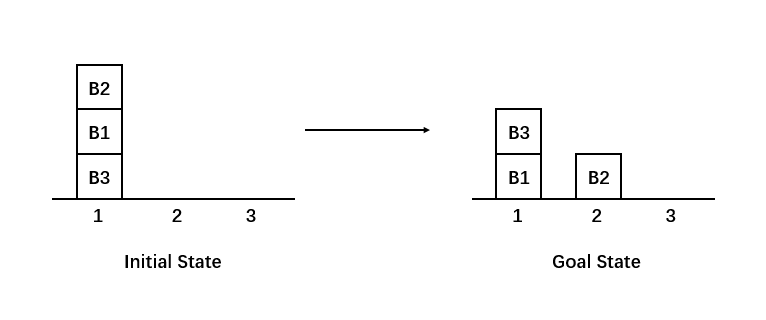
\includegraphics[width=15cm]{Pic/blocks1}
  \caption{Blocks World Case 1}
  \label{fig:blocks1}
\end{figure}
\begin{figure}[htbp]
  \centering
  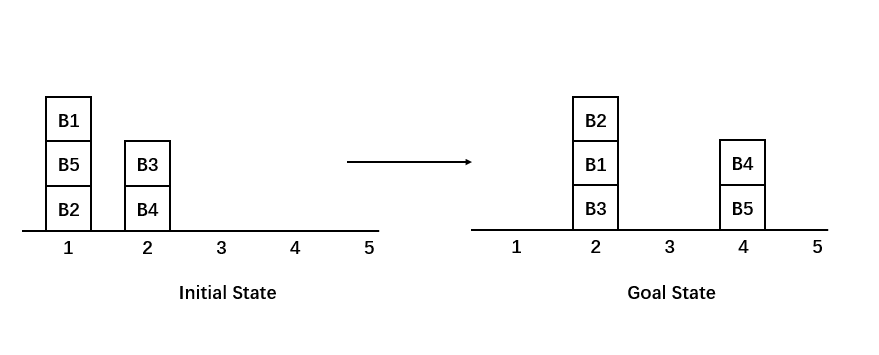
\includegraphics[width=17cm]{Pic/blocks2}
  \caption{Blocks World Case 2}
  \label{fig:blocks2}
\end{figure}\begin{figure}[htbp]
  \centering
  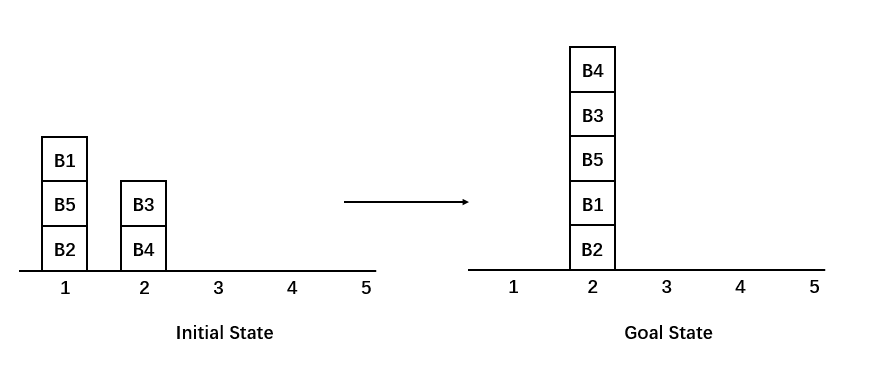
\includegraphics[width=15cm]{Pic/blocks3}
  \caption{Blocks World Case 3}
  \label{fig:blocks3}
\end{figure}\begin{figure}[ht]
  \centering
  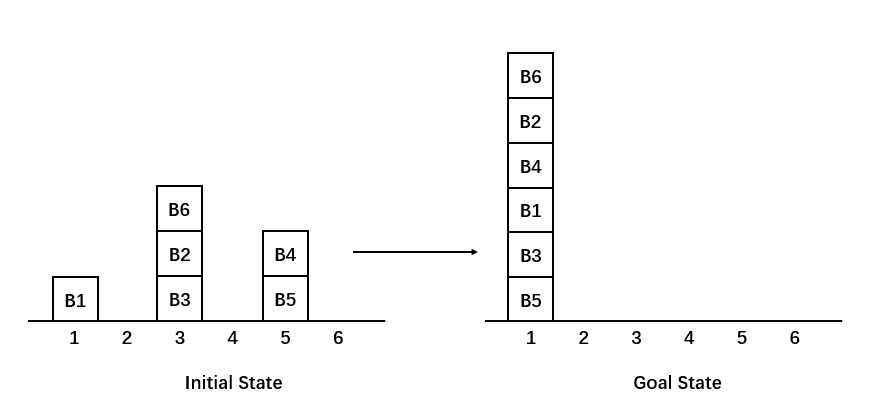
\includegraphics[width=15cm]{Pic/blocks4}
  \caption{Blocks World Case 4}
  \label{fig:blocks4}
\end{figure}\begin{figure}[ht]
  \centering
  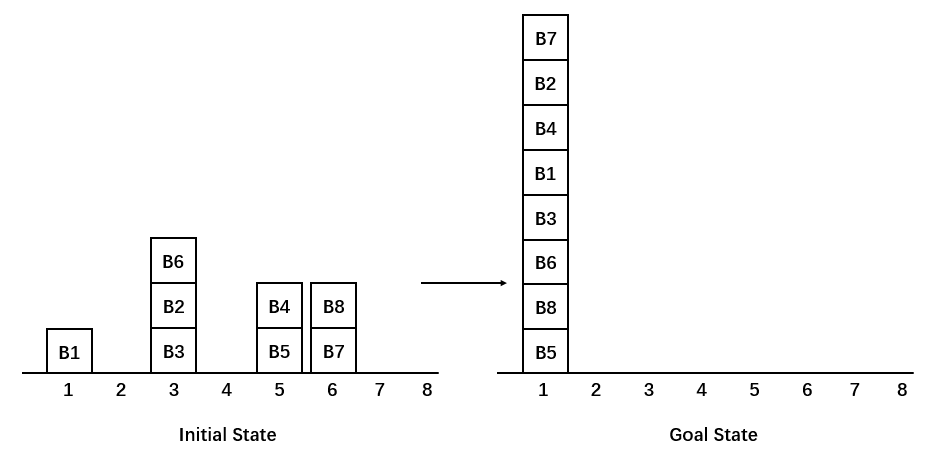
\includegraphics[width=13cm]{Pic/blocks5}
  \caption{Blocks World Case 5}
  \label{fig:blocks5}
\end{figure}
\section{Notes}
\begin{itemize}

\item Please send \textbf{P02\_YourNumber.zip} to the mailbox (\textbf{ai\_201901@foxmail.com}) before the deadline (\textbf{2019/10/30 23:59}). The \texttt{zip} file should contain several files: \textbf{futoshiki\_gac.cpp} or \textbf{futoshiki\_gac.py}, \textbf{blocksworld.pl}, \textbf{results pictures} and \textbf{other necessary files}, such as data files and README. 
\item Last but not least, you are not alone! If you find yourself stuck on something, contact the TA for help.

\end{itemize}



%\clearpage
%\bibliography{E:/Papers/LiuLab}
%\bibliographystyle{apalike}
\end{document} 
%%% Local Variables:
%%% mode: latex
%%% TeX-master: t
%%% End:
